\documentclass{article}
\usepackage[utf8]{inputenc}

% \title{Group of Seven Report}
% \author{1756850 Alkhamra, Othman Bader \\
% 1739256 Benicek, David \\
% 1770922 Bari, Aadam Ali \\
% 1425704 Mankani Vinod, Hitesh \\
% 1755013 Obimma, Timothy Uzochukwu \\ 
% 1783087 Vaddiraju, Nagarjuna}
% \date{January 2018}

\usepackage{natbib}
\usepackage{graphicx}
\usepackage{url}

\begin{document}
	
	\begin{titlepage}
		\newcommand{\HRule}{\rule{\linewidth}{0.5mm}} % Defines a new command for horizontal lines, change thickness here
		\newcommand{\hRule}{\rule{\linewidth}{0.1mm}} % Defines a new command for horizontal lines, change thickness here
		\centering
		
\includegraphics[width=0.2\textwidth]{kcl.png}\par\vspace{1cm}
		\textsc{\LARGE King's College London}\\[1.5cm] % Main heading such as the name of your university/college
		\textsc{\large 7CCSMGPR}\\[0.5cm] % Major heading such as course name
		\textsc{\Large Group Project}\\[0.5cm] % Minor heading such as course title
		\HRule\\[0.4cm]
		{\huge\bfseries Group of Seven Report}\\[0.4cm] % Title of your document
		\HRule\\[1.5cm]
		\vspace{1cm}
		\textit{Authors: }\vspace{0.5cm}
		\begin{center}
			\begin{tabular}{ c|c|c } 
				\hline
				\textbf{Number} & \textbf{Name} & \textbf{Email} \\
				\hline
				1756850 & Othman \textsc{Alkhamra} &  othman.alkhamra@kcl.ac.uk \\ 
				\hline
				1739256 & David \textsc{Benicek} &  david.benicek@kcl.ac.uk \\ 
				\hline
				1770922 & Aadam \textsc{Bari} &  
				aadam.bari@kcl.ac.uk\\ 
				\hline
				1425704 & Hitesh \textsc{Mankani Vinod} &  hitesh.mankani\_vinod@kcl.ac.uk \\ 
				\hline
				1755013 & Timothy \textsc{Obimma} &  timothy.obimma@kcl.ac.uk \\ 
				\hline
				1783087 & Nagarjuna \textsc{Vaddiraju} &  nagarjuna.vaddiraju@kcl.ac.uk \\ 
				
				\hline
			\end{tabular}
		\end{center}
		
		\vfill
		supervised by\par
		Dr.~Laurence \textsc{Tratt}\\
		\vfill
		{\large \today\par}
	\end{titlepage}
	% \maketitle
	\newpage
	\pagenumbering{roman}
	\tableofcontents
	\newpage
	\pagenumbering{arabic}
	\section{Introduction}
	In real life, we have different objects such as spheres, cubes ... etc. What is common between them is that they are all geometry objects. However, those objects might appear in different ways, based on their environment. For example, a glass sphere placed in an environment with many light sources will react in a different way than a metal sphere. And so, it is clear that different factors such as the material type, light sources and many other factors, will produce many different outputs. \\
	\par Ray tracing is one of those techniques which helps in producing different images for different environment variables. It is widely used in producing films, video games, animations, ... etc. It can be applied on any object and not just geometry objects.
	\subsection{What is the Idea behind  Ray Tracing?}
	Before discussing the idea behind ray tracing, and explaining its algorithm. Let's begin with listing the basic required elements to run the ray tracing algorithm. Those elements will be in one container which will be called \textbf{scene}. The elements of the scene are:
	\begin{itemize}
		\item \textbf{Object(s)}: a scene can contain one or many objects. Each object can be one of the previously mentioned objects or any other object, which exists in real life. For example, an object could be a sphere, triangle, tree, car, building ... etc.
		\item \textbf{Light source(s)}: The algorithm of ray tracing itself doesn't require having a light source. However, a scene without any light source, won't make the use of ray tracing effective.
		\item \textbf{Image Plane}: which is called \textbf{window frame} in our implementation. This plane will have some width and height, and it will be divided into small squares, and each square will be covering a number of pixels on the objects of the scene.
		\item \textbf{Eye or Camera:} In order to render the scene, it is mandatory to have an eye or camera, with some position and some direction, to detect the way of looking to the scene elements. From that eye or camera, rays will be produced, and will go through the image plane.
	\end{itemize}
	\begin{figure}[ht!]
		\centering
		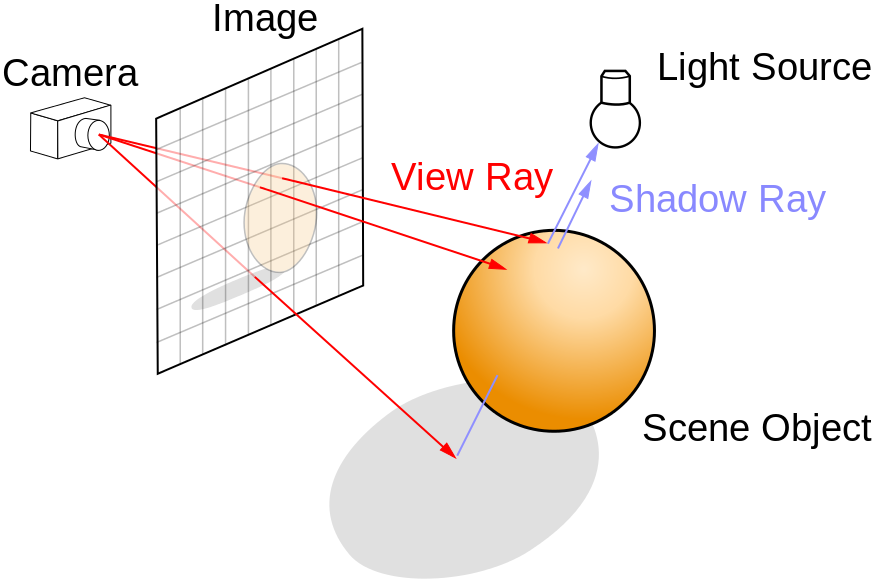
\includegraphics[scale=0.30]{./raytracing.png}
		\caption{Ray Tracing's Scene Elements \cite{raytracingpic}}
		\label{fig:raytracing}
	\end{figure}
	\par \textbf{Figure \ref{fig:raytracing}} shows an example of a scene with the previously listed elements. Now, and after discussing the elements of the scene, it is the time to describe the algorithm of ray tracing. The idea is so simple, in each scene there will an eye or camera, from that camera many rays will be produced and go across the small squares in the image plane, for each ray we need to check whether it intersects with any of the objects or not, and return the color of that pixel.\\
	\par The algorithm itself is really simple. Nevertheless, it is previously mentioned that environment variables play a big role in the calculations. And so, returning the color of the pixel, which was hit by the the ray, won't be that simple; since it will require additional computations related to the reflections, shades ... etc. 
	\subsection{Our Solution}
	Although the idea behind ray tracing is simple. But, there are many different problems to be addressed in this program. These problems can be summarized as below:
	\subsubsection{Web Interface}
	In order to define the different elements of the scene, a web interface is developed to allow users enter the different values for the scene elements. Using this interface, the user can add different objects to the scene, with different materials, positions, sizes, colors. Furthermore, adding different lights at different positions with different colors. \\
	\par The challenge here is that objects must be in 3D. And so, we developed a web interface with two options. One option is the 2D option, where the user needs to define an element by providing its values in the top and side views. The other option, is the 3D view, where the user can add elements directly in 3D format.\\
	\par All the functionalities in our web interface support the drag and drop feature. In other words, this means that the user can define the position by clicking on the object, and moving it in any direction.
	\subsubsection{Ray tracing Engine}
	The other part of our system is the backend engine, where all the calculations are done based on the input received from the web interface. This system was developed using .NET C\#. It includes a post API, which will receive the request from the client, and it is able to render a scene with the followings:
	\begin{itemize}
		\item A scene with the following objects:
		\begin{itemize}
			\item \textbf{Plane}: This object will be used to create the walls in the scene. And it will have position, and a normal which will decide the orientation, in addititon to one of the supported materials.
			\item \textbf{Cube}: Each cube will have a size, a position, and one of the supported materials.
			\item \textbf{Sphere}: Each sphere will have a radius, center point, and one of the supported materials.
		\end{itemize}
		The  \textbf{supported materials} are:
		\begin{itemize}
			\item \textbf{Phong materials}:  which will follow the phong theory such as chalk, metal, plastic. The difference between those materials are the different values of diffusion, specular coefficients and the light color infulence.
			\item \textbf{Flat material}: which is the simplest material, which will return the color of that object regardless to any other environment variables and parameters.
			\item \textbf {Glass material}: this material is the most complicated one, which will do many different calculations in order to calculate the color of each pixel of that object.
		\end{itemize}
		Each of these materials can have a color chosen by the user, or just use the default color, if \textbf{nothing} is received.
		\item A scene with multiple light sources at different positions and different colors.
		\item A scene with perspective camera, this camera will have the position, the direction of how to look at the image plane, and the distance from that plane.
	\end{itemize}
	\section{Review}
	\section{Requirements and design}
	\section{Implementation}
	\subsection{Front End}
	\subsection{Backend}
	\subsubsection{Unit Testing}
	\section{Team work}
	\section{Evaluation}
	
	\clearpage
	\bibliographystyle{plain}
	\bibliography{references}
\end{document}
